% \iffalse
\let\negmedspace\undefined
\let\negthickspace\undefined
\documentclass[journal,12pt,onecolumn]{IEEEtran}
\usepackage{cite}
\usepackage{amsmath,amssymb,amsfonts,amsthm}
\usepackage{algorithmic}
\usepackage{graphicx}
\usepackage{textcomp}
\usepackage{xcolor}
\usepackage{txfonts}
\usepackage{listings}
\usepackage{enumitem}
\usepackage{mathtools}
\usepackage{gensymb}
\usepackage{comment}
\usepackage[breaklinks=true]{hyperref}
\usepackage{tkz-euclide} 
\usepackage{listings}
\usepackage{gvv}    
\usepackage[italicdiff]{physics}
\usepackage{mathrsfs}
\def\inputGnumericTable{}                                 
\usepackage[latin1]{inputenc}                                
\usepackage{color}                                            
\usepackage{array}                                            
\usepackage{longtable}                                       
\usepackage{calc}                                             
\usepackage{multirow}                                         
\usepackage{hhline}                                           
\usepackage{ifthen}                                           
\usepackage{lscape}

\newtheorem{theorem}{Theorem}[section]
\newtheorem{problem}{Problem}
\newtheorem{proposition}{Proposition}[section]
\newtheorem{lemma}{Lemma}[section]
\newtheorem{corollary}[theorem]{Corollary}
\newtheorem{example}{Example}[section]
\newtheorem{definition}[problem]{Definition}
\newcommand{\BEQA}{\begin{eqnarray}}
\newcommand{\EEQA}{\end{eqnarray}}
\newcommand{\define}{\stackrel{\triangle}{=}}
\theoremstyle{remark}
\newtheorem{rem}{Remark}
\begin{document}
\bibliographystyle{IEEEtran}
\vspace{3cm}

\title{NCERT-discrete : 11.14 - 23}
\author{EE23BTECH11025 - Anantha Krishnan $^{}$% <-this % stops a space
}
\maketitle
\bigskip

\renewcommand{\thefigure}{\theenumi}
\renewcommand{\thetable}{\theenumi}

\section{question}
A circular disk of mass 10kg is suspended by a wire attached to its centre. The wire is twisted by rotating the disc and released. The period of torsional oscillations is found to be 1.5s. The radius of the disc is 15cm. Determine the torsional spring constant of the wire. (Torsional spring constant $\alpha$ is defined by the relation J=-$\alpha$$\theta$, where J is the restoring couple and $\theta$ is the angle of twist).\\

\textbf{Solution:}
    \begin{table}[ht!]
\centering
\begin{tabular}{ |c|c|c| } 
 \hline
Symbols & Description & Values  \\
\hline
 $T$ & Time period of a body following the law $x_{(t)} = a\sin{\omega t}$ &$\frac{2\pi}{\omega}$\\
 \hline
 $\alpha$ & Torsional constant & (?)\\
 \hline
 $m$ & Mass of pendulum & $9kg$\\
 \hline
 $r$& Radius of disc & $15cm$\\
 \hline
 $I$ & Moment of inertia of the disc & $0.1125kgm^{-2}$\\
\hline
\end{tabular}
\caption{Parameters, Descriptions, and Values}
\label{table:ee25-tab3}
\end{table}




A torsional pendulum is governed by the following law:
\begin{align}
    J &= -\alpha\theta(t) 
\end{align}
From $J = I\alpha$ and $\alpha = \dv[2]{\theta(t)}{t}$
\begin{align}
\dv[2]{\theta(t)}{t} + \frac{\alpha\theta(t)}{I} &= 0
\end{align}
For the Laplace transform of the differential : 
Assuming $\theta(0)$ = 0,
\begin{align}
0 &= s^2\mathscr{L}\brak{\theta(t)} - s\theta(0) - \theta'(0) + \frac{\alpha\mathscr{L}\brak{\theta(t)}}{I}\\
\mathscr{L}\brak{\theta(t)} &= \frac{\theta'(0)}{s^2+\frac{\alpha}{I}}
    \end{align}
For the Inverse Laplace transform of $\mathscr{L}\brak{\theta(t)}$: Using Bromwich integral,
\begin{align}
 \theta(t) &= \frac{1}{2\pi j}\int_{c-j\infty}^{c+j\infty}\mathscr{L}\brak{\theta(t)}e^{st}\,dt , c > 0\\
 &= \frac{1}{2\pi j}\int_{c-j\infty}^{c+j\infty}\frac{\theta'(0)e^{st}}{s^2+\frac{\alpha}{I}}\,dt
\end{align}
Since the poles $s=j\sqrt{\frac{\alpha}{I}}$ and $s=-j\sqrt{\frac{\alpha}{I}}$ (both non repeated, i.e. $m=1$) lie inside a semicircle for some $c>0$. Using Jordans lemma and method of residues from \ref{table:ee25-tab3} :
\begin{align}
      R_1&=\lim\limits_{s\to j\sqrt{\frac{\alpha}{I}}}\brak {{\brak{s-j\sqrt{\frac{\alpha}{I}}}}\brak{\frac{\theta'(0)}{s^2+\frac{\alpha}{I}}} e^{st}}\\
&={\brak{\frac{\theta'(0)Ie^{j\sqrt{\frac{\alpha}{I}}t}}{2j\alpha}}}\\
  R_2&=\lim\limits_{s\to -j\sqrt{\frac{\alpha}{I}}}\brak {{\brak{s+j\sqrt{\frac{\alpha}{I}}}}\brak{\frac{\theta'(0)}{s^2+\frac{\alpha}{I}}} e^{st}}\\
&={\brak{\frac{-\theta'(0)Ie^{-j\sqrt{\frac{\alpha}{I}}t}}{2j\alpha}}}\\
\theta(t) &= R_1 + R_2\\
\theta(t) &= {\brak{\frac{\theta'(0)I\brak{e^{j\sqrt{\frac{\alpha}{I}}t}-e^{-j\sqrt{\frac{\alpha}{I}}t}}}{2j\alpha}}}\\
\implies
\theta(t) &=\theta'(0)\sin{\brak{t\sqrt{\frac{\alpha}{I}}}}
\end{align}
For calculating the torsional constant :
From table \ref{table:ee25-tab3}.
\begin{align}
 T &= 2\pi\sqrt{\frac{I}{\alpha}}\\
\implies \alpha &= 1.972 Nms^{-1}
\end{align}

    \begin{figure}[!ht]    
    \centering
\graphicspath{ {figs/} }
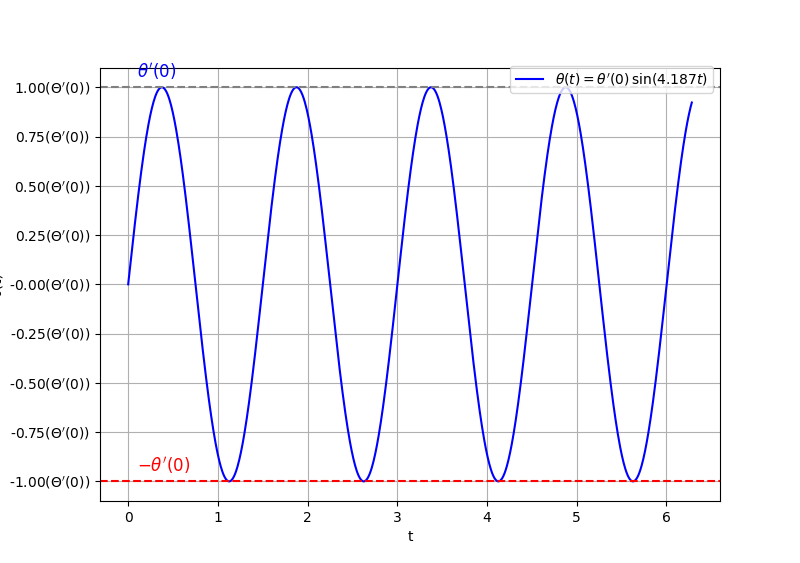
\includegraphics[width=\columnwidth]{graph_1}
\caption{ $\theta(t)$ vs t }
\label{graph:ee25-g4}
\end{figure}











\end{document}
